\chapter{Introduction}
\label{Chapter1}
\lhead{Chapter 1. \emph{Introduction}}

\section{Background and Motivation}

Thermal imaging captures infrared radiation emitted by objects, enabling temperature-based analysis that is robust to varying illumination, smoke, and adverse weather conditions. This sensing modality is critical across a wide range of high-value applications: surveillance systems that must function in complete darkness, medical diagnostics that map inflammatory patterns, and precision agriculture that detects plant stress before visual symptoms appear. Despite these advantages, the deployment of thermal imaging in data-driven machine learning pipelines is severely constrained by two fundamental factors.

First, Long-Wave Infrared (LWIR) thermal cameras are prohibitively expensive. A research-grade FLIR thermal camera costs between \$3,000 and \$80,000 USD, placing this technology far outside the reach of farmers, community health workers, and small-scale security operators. Second, even when cameras are available, the collection of large annotated \emph{paired} datasets --- where each RGB photograph has a corresponding thermal image of the same scene at the same instant --- is logistically demanding. Existing public datasets in this space contain only a few thousand paired samples, which is insufficient to train modern deep architectures from scratch without regularisation.

These two constraints together motivate a compelling research question: \emph{Can a deep learning model synthesise a realistic thermal image directly from a cheap, abundant RGB photograph?} If so, thermal imaging becomes accessible without physical cameras, and the scarcity problem is partially solved through data augmentation.

\section{Problem Definition}

The task is formally a \textbf{cross-modal image-to-image translation}: given an RGB image $\mathbf{x} \in \mathbb{R}^{3 \times H \times W}$, learn a mapping $G: \mathbf{x} \mapsto \hat{\mathbf{y}}$ such that the synthesised thermal image $\hat{\mathbf{y}} \in \mathbb{R}^{1 \times H \times W}$ is structurally consistent with the ground-truth thermal image $\mathbf{y}$.

This mapping is fundamentally non-trivial because:
\begin{itemize}
    \item The RGB-to-thermal relationship is physically governed by the heat diffusion PDE $\partial T/\partial t = \alpha \nabla^2 T$, which imposes smooth spatial gradients and energy conservation constraints that an unconstrained network need not satisfy.
    \item Multiple RGB images may map to similar yet thermally distinct outputs (e.g., healthy vs. stressed leaves look similar in RGB but have very different infrared signatures).
    \item The frequency-domain structure of thermal images is fundamentally different from RGB: thermal images are low-frequency dominant because heat diffuses smoothly, while RGB images contain rich high-frequency texture.
\end{itemize}

Standard image translation frameworks such as pix2pix~\cite{b_pix2pix} and CycleGAN~\cite{b_cyclegan} do not incorporate any of these domain-specific physical priors, and standard Generative Adversarial Networks (GANs) frequently produce artefacts, mode collapse, or thermally implausible outputs when applied naively to this domain.

\section{Proposed Solution}

This work proposes \textbf{PC-LiquidGAN} (Physics-Constrained LiquidGAN), building upon the base \textbf{LiquidGAN} framework of Sarath and Nair~\cite{b_liquidgan} with four novel contributions:

\begin{enumerate}
    \item \textbf{ODE-UNet Generator:} A Neural ODE-based UNet with spatial skip connections replaces the flat-latent ODE generator of the base paper. The ConvODE bottleneck models continuous thermal diffusion dynamics on 2D spatial feature maps, while skip connections prevent spatial information loss.
    \item \textbf{Adaptive ODE Solver (dopri5):} The Dormand-Prince 4/5th-order adaptive solver replaces the fixed RK4 solver of the base paper, allocating more function evaluations to thermally complex spatial regions.
    \item \textbf{Heat Diffusion PDE Loss:} A physics-informed loss enforcing the residual of $\partial T/\partial t = \alpha \nabla^2 T$ explicitly penalises thermodynamically implausible outputs.
    \item \textbf{FFT Spectral Loss:} A frequency-domain loss with a Gaussian low-frequency emphasis mask forces the generator to match the thermal frequency signature of real images.
\end{enumerate}

The Liquid Neural Network (LNN) discriminator~\cite{b_lnn} is retained from the base paper with its learnable time constants for adaptive thermal texture discrimination.

\begin{figure}[htbp]
    \centering
    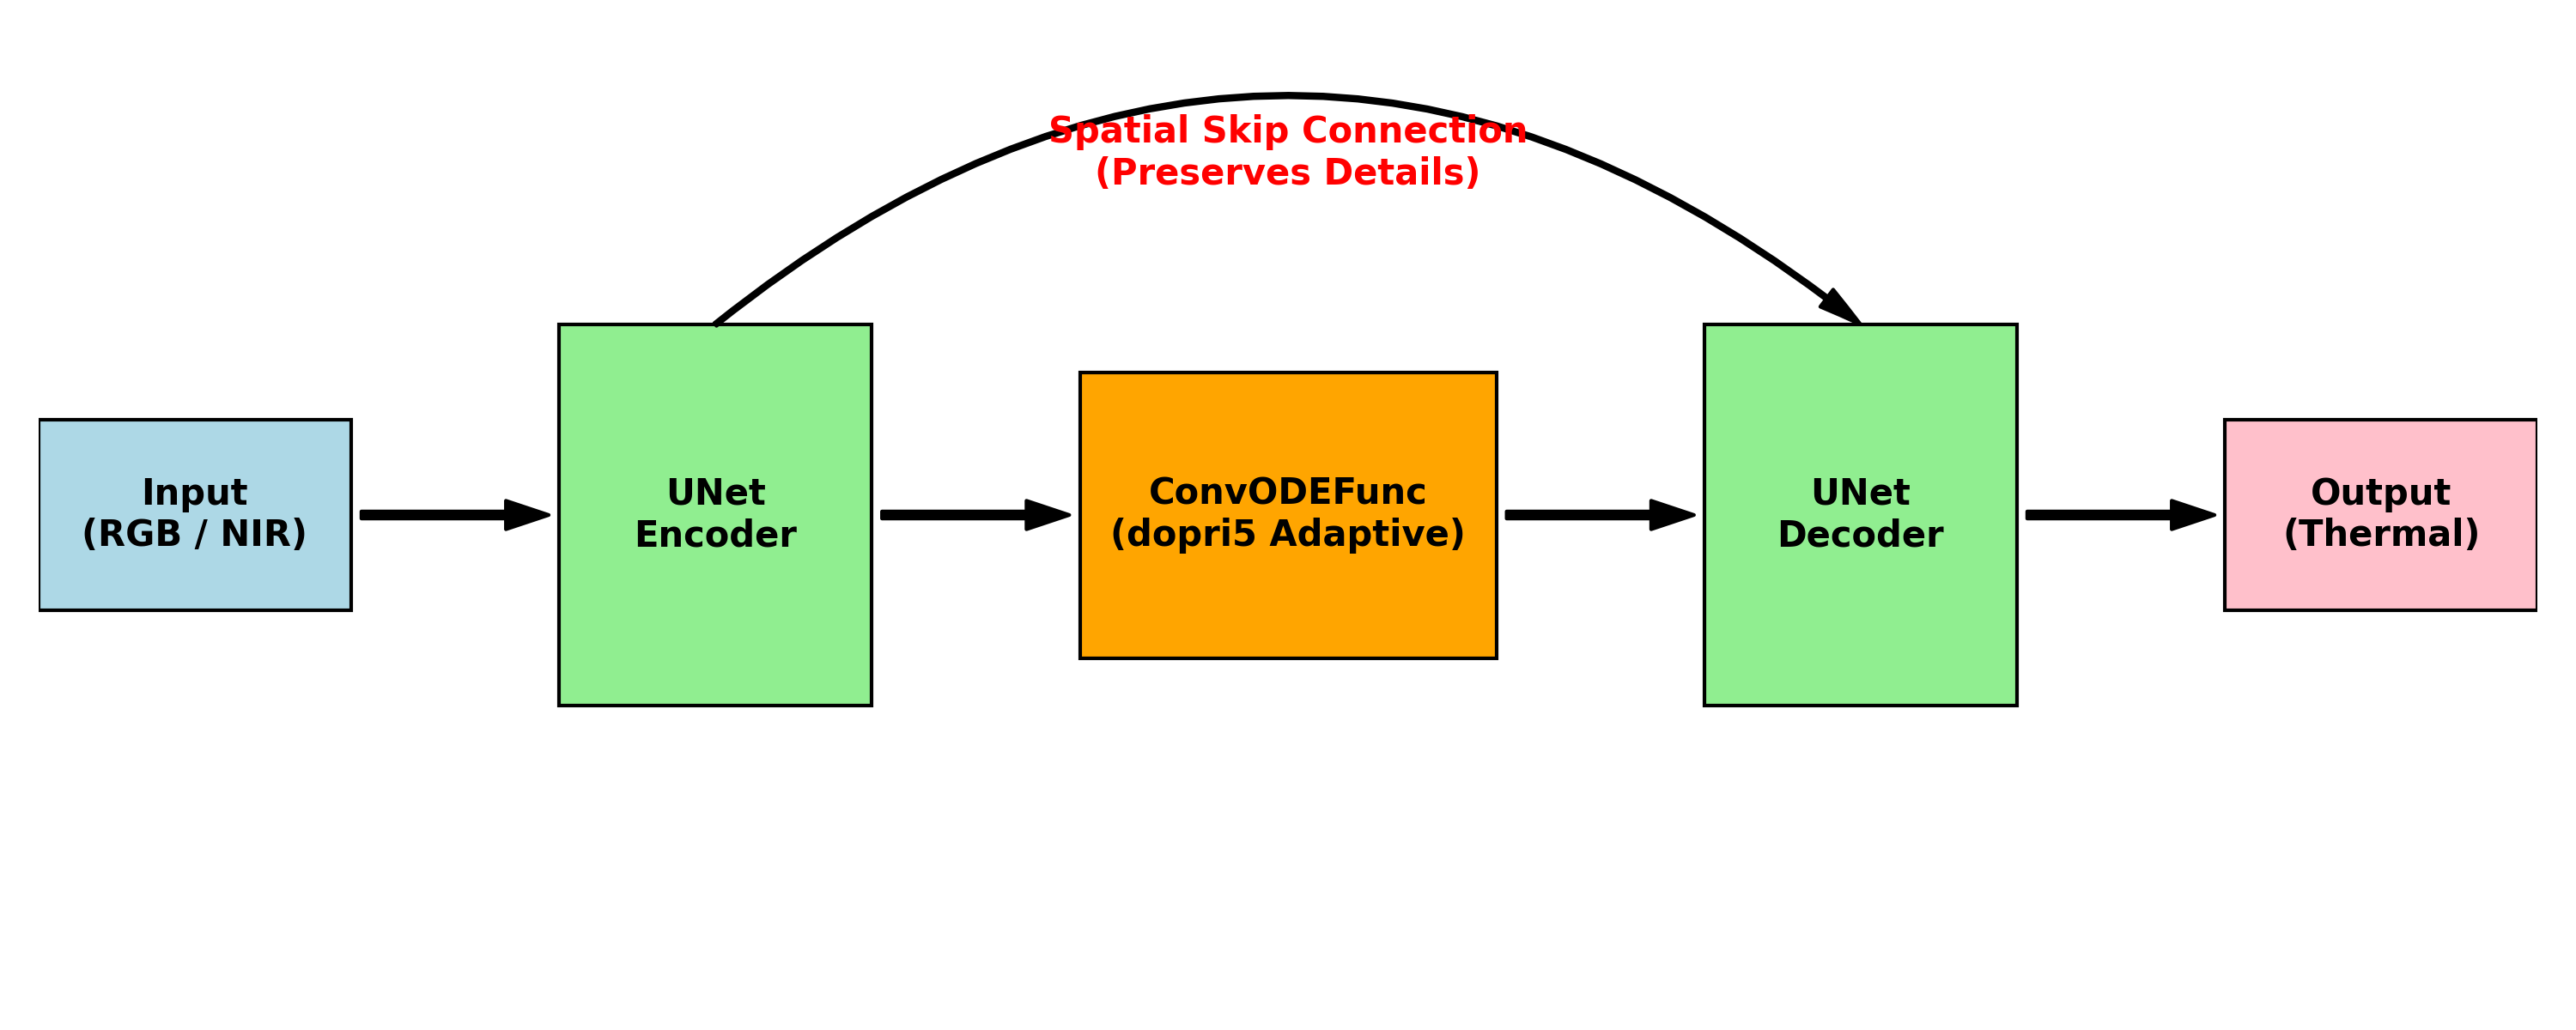
\includegraphics[width=\linewidth]{architecture.png}
    \caption{High-level architecture of PC-LiquidGAN showing the ODE-UNet Generator with spatial skip connections, the Liquid Neural Network Discriminator, and the two physics-informed loss terms (heat diffusion PDE and FFT spectral matching).}
    \label{fig:arch_overview}
\end{figure}

\section{Objectives}

The primary objectives of this project are:
\begin{itemize}
    \item To integrate physics-aware constraints derived from the heat diffusion PDE into an adversarial training framework for thermal image synthesis.
    \item To evaluate the benefit of adaptive ODE solvers over fixed-step solvers for spatial thermal dynamics modelling.
    \item To demonstrate that FFT spectral matching significantly improves the low-frequency fidelity of synthesised thermal images.
    \item To validate the model across five diverse cross-domain thermal datasets, including surveillance, medical, biometric, and agricultural domains.
    \item To perform a comprehensive ablation study confirming the independent contribution of each proposed component.
    \item To evaluate zero-shot cross-domain generalisation of the physics-informed model without per-domain fine-tuning.
\end{itemize}

\section{Scope and Limitations}

This work focuses exclusively on paired RGB-to-thermal translation (supervised setting). The model is trained independently per domain and does not use domain adaptation or fine-tuning for zero-shot evaluation. The physics loss uses a fixed thermal diffusivity constant $\alpha = 0.001$ rather than a spatially-varying learned map. All experiments are performed at $256 \times 256$ pixel resolution.

\section{Report Organisation}

The remainder of this report is organised as follows. Chapter~\ref{Chapter2} reviews the literature on GANs, Neural ODEs, Liquid Neural Networks, and physics-informed learning. Chapter~\ref{Chapter3} details the proposed PC-LiquidGAN methodology and loss formulation. Chapter~\ref{Chapter4} describes the generator and discriminator architectures in detail. Chapter~\ref{Chapter5} presents the experimental setup, datasets, and main quantitative results. Chapter~\ref{Chapter6} presents the ablation study and solver comparison. Chapter~\ref{Chapter7} concludes the report and discusses future directions. Appendices provide hyperparameter tables, dataset details, and representative code listings.
